\section{Multiplicity-sensitive upper-bound arguments}
\label{upper:scope}

This section develops upper estimates by separating ordinary crossings from finite multiple points. Actual elementary segments, incidence, clean-line charging and classical simple bounds were completed in the preceding release. The 5--6 October development additionally extracts cyclic fans, side matching, shared-core components and geometric escape from the real arrangement. The final structural theorems therefore have no supplied fan or aggregate budget premise. Their class restrictions and residual corrections remain explicit; they are not improved unrestricted numerical bounds for $\K$ depending only on the line count.

The distinction is necessary because the even-order estimates of Bartholdi--Blanc--Loisel and Blanc require simplicity~\citep{bbl2008,blanc2011}. The classical Cl\'ement--Bader envelope is treated as a reported external theorem~\citep{clementbader2007}; the local example in Section~\ref{upper:shared-fan} explains why we do not silently replace its proof by a bound on all shared edges incident to a multiple point.

\subsection{An exact elementary-segment identity}

\begin{definition}
For an arrangement of $n$ distinct affine lines, let $t_r$ be the number of finite intersection points incident to exactly $r$ lines, and let $P$ be the number of unordered parallel pairs. A bounded \emph{elementary segment} is the portion of an arrangement line between two consecutive finite intersection points. Let $E$ count these segments, $U$ count those incident to no triangular cell, and $D$ count those incident to two triangular cells. Let $a$ be the number of lines containing at least one finite intersection point, and put
\[
 S=\sum_{r\ge3}r(r-2)t_r,\qquad
 \delta=n(n-2)-3T,
\]
where $T$ is the number of bounded triangular cells.
\end{definition}

\begin{proposition}[Segment and defect identities]
\label{upper:identity}
For every such arrangement,
\begin{align}
 E&=n(n-1)-2P-S-a,\\
 3T&=E-U+D,\\
 \delta&=2P+S+a-n+U-D.
 \label{upper:defect-general}
\end{align}
If every line meets another line, then $a=n$ and $\delta=2P+S+U-D$.
\end{proposition}

\begin{proof}
Each nonparallel unordered pair contributes to exactly one finite point, so
\[
 n(n-1)-2P=\sum_{r\ge2}r(r-1)t_r.
\]
If a line has $s>0$ distinct finite intersection points, it contributes $s-1$ bounded elementary segments; an isolated line contributes none. Summing point-line incidences gives
\[
 E=\sum_{r\ge2}r t_r-a.
\]
Subtracting these expressions yields the first identity. Each triangular cell uses three elementary segments. A segment is incident to zero, one, or two such cells, so the total number of triangle-side incidences is $E-U+D$. Substitution into the definition of $\delta$ gives the last identity.
\end{proof}

The term $D$ cannot be dropped in a nonsimple arrangement. Multiple points reduce the available segment count by $S$, but sharing can compensate for some of that loss. This is precisely the interaction that a classical upper proof must control.

\begin{lemma}[A shared side has a multiple endpoint]
\label{upper:shared-endpoint}
An elementary segment incident to two bounded triangular cells cannot have both endpoints ordinary, where an ordinary point is incident to exactly two arrangement lines.
\end{lemma}

\begin{proof}
At each ordinary endpoint there is a unique supporting line other than the line containing the segment. Both adjacent triangles would therefore have the same three supporting lines. Three distinct lines have at most one bounded triangular region, whereas the two incident cells lie on opposite sides of the shared segment. This is impossible.
\end{proof}

The parity estimates below assume even $n\ge4$ and pairwise nonparallel lines. The later component statements hold for either parity at $n\ge2$. Let the \emph{core} consist of the finite points of multiplicity at least three. Write
\[
 q=\sum_{r\ge3}t_r,\qquad I=\sum_{r\ge3}r t_r,
\]
and let $h$ count the lines meeting the core. Let $D_1$ count shared elementary segments with exactly one core endpoint and $D_2$ those with two core endpoints. By Lemma~\ref{upper:shared-endpoint}, $D=D_1+D_2$, and hence
\begin{equation}
 \delta=S+U-D_1-D_2.
 \label{upper:core-identity}
\end{equation}

\subsection{Parity on a line outside the core}

A line is \emph{clean} if it contains no core point. The following argument adapts the local parity method in Blanc's Section~2~\citep{blanc2011}. Its proof is included because the transverse lines may have multiple intersections away from the clean line.

\begin{lemma}[Clean-line charging]
\label{upper:clean-charge}
For even $n\ge4$ and pairwise nonparallel lines,
\begin{equation}
 n-h\le2U+D_1.
 \label{upper:charging}
\end{equation}
\end{lemma}

\begin{proof}
First fix a clean line $L$, place it horizontally, and number its $n-1$ crossings from left to right. Let $R_i$ be the transverse line at crossing $i$. Denote the bounded segment of $L$ between crossings $i$ and $i+1$ by $\ell_i$, and its two exterior rays by $\ell_0$ and $\ell_{n-1}$. Write $p_i^+$ and $p_i^-$ for the faces above and below $\ell_i$, and $r_i^+,r_i^-$ for the elementary transverse pieces of $R_i$ immediately above and below $L$. A transverse piece may be a bounded segment or an unbounded ray.

We show that some bounded $r_i^{\pm}$ is unused or shared. Suppose otherwise: every bounded transverse piece is incident to exactly one triangle. Each bounded $\ell_i$ is unshared by Lemma~\ref{upper:shared-endpoint}.

If both $p_1^+$ and $p_1^-$ are nontriangular, then $r_1^+$ and $r_1^-$ are unused: their other adjacent faces meet the exterior ray $\ell_0$. At least one of these transverse pieces is bounded, because $R_1$ meets another transverse line. This contradicts the supposition. Reflecting across $L$ if necessary, assume $p_1^+$ is triangular; $p_1^-$ is then not.

For $1\le i\le n-2$, prove the following assertions together:
\begin{enumerate}[label=(\roman*)]
\item if $i$ is even, $p_i^+$ is nontriangular; if $i$ is odd, $p_i^-$ is nontriangular;
\item if both faces at $\ell_{i-1}$ are nontriangular, then $p_i^-$ is triangular for even $i$, and $p_i^+$ is triangular for odd $i$.
\end{enumerate}
The base case follows from the choice of $p_1^+$ and the unbounded faces at $\ell_0$. Consider an even step; the odd step exchanges signs. If $p_{i-1}^+$ is triangular, then $p_i^+$ cannot be triangular, since otherwise the two triangles share the bounded piece $r_i^+$, contrary to the supposition. Assertion (ii) has a false antecedent in this case.

Otherwise both $p_{i-1}^+$ and $p_{i-1}^-$ are nontriangular by the preceding odd step. This cannot happen for $i=2$, so $i\ge4$. The earlier even step makes $p_{i-2}^+$ nontriangular. Hence $r_{i-1}^+$ is unused, and must be unbounded. The intersection of $R_{i-1}$ and $R_i$ must consequently lie below $L$. It follows that $r_i^-$ is bounded. Its left adjacent face is nontriangular, so its right adjacent face $p_i^-$ must be triangular. Since $\ell_i$ is unshared, $p_i^+$ is nontriangular. This proves both assertions.

Now $n-2$ is even, so $p_{n-2}^+$ is nontriangular. If $p_{n-2}^-$ is also nontriangular, both pieces at the last crossing are unused and at least one is bounded, again a contradiction. Otherwise $p_1^+$ and $p_{n-2}^-$ are triangular, while $r_1^-$ and $r_{n-1}^+$ are unused. The lines $R_1$ and $R_{n-1}$ intersect. If their intersection is below $L$, then $r_1^-$ is bounded; if above, then $r_{n-1}^+$ is bounded. This is the final contradiction.

Charge each clean line to one bounded unused or shared transverse segment supplied by this argument. An unused segment can receive at most two charges, one at each ordinary endpoint. A shared segment must have a multiple endpoint, so it can receive at most one charge if counted by $D_1$, and none if counted by $D_2$. There are $n-h$ clean lines, giving~\eqref{upper:charging}.
\end{proof}

\begin{remark}[Why parallel pairs have been excluded]
Three parallel vertical lines and one horizontal line give a clean horizontal line whose transverse pieces are all unbounded. Thus simply removing parallel-participating lines from the set to be charged does not prove the lemma. The identities of Proposition~\ref{upper:identity} allow parallels, but the charging argument above does not. Every subsequent upper estimate in this section retains the pairwise nonparallel hypothesis.
\end{remark}

Combining~\eqref{upper:core-identity} and~\eqref{upper:charging} gives the basic budget
\begin{equation}
 2\delta\ge n+2S-h-3D_1-2D_2.
 \label{upper:basic-budget}
\end{equation}
The remaining problem is to bound the shared-side contribution at the core.

\subsection{The geometric obstruction in a cyclic fan}

At an $r$-fold point $v$, the incident lines determine $2r$ rays in cyclic order, with opposite rays separated by $r$ positions. Let $d_1(v)$ count shared elementary segments starting at $v$ and ending at an ordinary point, and let $d_2(v)$ count those ending at another core point. A ray supports at most one such incident elementary segment.

\begin{lemma}[No long run of ordinary-ended shared rays]
\label{upper:no-long-run}
For $r\ge3$, no $r-1$ consecutive rays at an $r$-fold point can all support segments counted by $d_1(v)$.
\end{lemma}

\begin{proof}
Such a run would border $r$ consecutive triangular sectors. At the ordinary endpoint of each selected shared segment, the opposite supporting lines of the two neighboring triangles must coincide: besides the radial line through $v$, only one arrangement line passes through that endpoint. Propagating this equality makes the opposite sides of all $r$ triangles lie on one line $M$.

The line $M$ would meet $r+1$ consecutive rays from $v$, which include an opposite pair. A line meeting both open opposite rays must contain their connecting segment and hence $v$. But the opposite side of a nondegenerate triangle with vertex $v$ cannot lie on a line through $v$. This contradiction proves the lemma.
\end{proof}

This is an actual geometric statement, not an assumed combinatorial prohibition. The Lean module \texttt{FanGeometry} proves uniqueness and propagation of opposite supports for real lines and points. The module \texttt{CyclicFan} supplies the cyclic-to-geometric bridge from triangular sectors, antipodal rays and ordinary selected endpoints.

\begin{proposition}[Local fan budget]
\label{upper:fan-budget}
At every finite point of multiplicity $r\ge3$,
\begin{equation}
 d_1(v)\le2r-3,\qquad 3d_1(v)+d_2(v)\le6r-6.
 \label{upper:local-fan-budget}
\end{equation}
\end{proposition}

\begin{proof}
Count selected rays in all $2r$ cyclic windows of length $r-1$. Each window contains at most $r-2$ selected rays by Lemma~\ref{upper:no-long-run}, and each selected ray belongs to exactly $r-1$ windows. Therefore
\[
 (r-1)d_1(v)\le2r(r-2).
\]
If $d_1(v)\ge2r-2$, the left side is at least $2(r-1)^2=2r(r-2)+2$, a contradiction. Finally $d_1(v)+d_2(v)\le2r$, so
\[
 3d_1(v)+d_2(v)=2d_1(v)+(d_1(v)+d_2(v))\le6r-6.
\]
\end{proof}

The cyclic double count is proved in \texttt{FanCount}. The theorem \lean{CyclicFan.selected_card_le} combines it with the real geometric obstruction, without assuming the no-long-run conclusion as an unexplained premise.

\subsection{A weighted bound for an arbitrary finite core}

\begin{proposition}[Multiplicity-weighted defect estimate]
\label{upper:weighted}
Let $n\ge4$ be even and let the arrangement be pairwise nonparallel. Then
\begin{equation}
 2\delta\ge n+\sum_{r\ge3}(2r^2-11r+6)t_r.
 \label{upper:weighted-defect}
\end{equation}
\end{proposition}

\begin{proof}
Each $D_1$ segment has exactly one core endpoint and each $D_2$ segment has two. Summing~\eqref{upper:local-fan-budget} gives
\[
 3D_1+2D_2\le6I-6q.
\]
Also $h\le I$, since every core line contributes at least one point-line incidence. Inserting both inequalities into~\eqref{upper:basic-budget} yields
\[
 2\delta\ge n+2S-7I+6q,
\]
which is~\eqref{upper:weighted-defect} after expanding $S,I,q$.
\end{proof}

The local weights are $-9,-6,1,12,27$ at multiplicities $3,4,5,6,7$, respectively. Consequently the obstruction to recovering a simple-style parity defect is concentrated at triple and quadruple points; higher multiplicity has a positive weight in this accounting.

\begin{corollary}[Nonnegative core weight]
\label{upper:high-multiplicity}
Under the hypotheses of Proposition~\ref{upper:weighted}, if
\[
 \sum_{r\ge3}(2r^2-11r+6)t_r\ge0,
\]
then
\[
 T\le\left\lfloor\frac{n(n-5/2)}3\right\rfloor.
\]
In particular, this holds if every finite multiple point has multiplicity at least five.
\end{corollary}

\begin{proof}
The weighted estimate implies $\delta\ge n/2$, giving the displayed upper bound by the definition of $\delta$. For $r\ge5$, the exact factorization
\[
 2r^2-11r+6=1+(r-5)(2r-1)\ge1
\]
proves the stated sufficient condition.
\end{proof}

This extends the same polynomial to a restricted nonsimple class. It says nothing comparable for a general core consisting of many triple points. Numerical first priority for this restricted consequence has not been established.

\subsection{A sharper estimate with at most two core points}

\begin{lemma}[A fan with at most one core-to-core ray]
\label{upper:one-core-ray}
If $d_2(v)\le1$ at a point of multiplicity $r\ge3$, then $d_1(v)\le2r-4$.
\end{lemma}

\begin{proof}
Mark which of the $2r$ sectors at $v$ are triangular. A ray supports a shared elementary segment exactly when both neighboring sectors are triangular. If every sector is triangular, every ray is shared; deleting at most one $d_2$ ray leaves a run of at least $2r-1$ selected rays, contradicting Lemma~\ref{upper:no-long-run}. Hence a nontriangular sector exists.

Suppose $d_1(v)\ge2r-3$. Two separated nontriangular sectors exclude at least four shared rays, as do three consecutive nontriangular sectors. Both situations are impossible. If exactly one sector is nontriangular, the shared rays form a path of length $2r-2$. Deleting at most one $d_2$ ray leaves at most two selected runs. Their total capacity is $2(r-2)$, less than the required $2r-3$. If exactly two adjacent sectors are nontriangular, at most $2r-3$ shared rays remain. All would have to be selected, forming a run of length $2r-3>r-2$. These cases exhaust the possibilities and prove the lemma.
\end{proof}

\begin{theorem}[At most two finite multiple points]
\label{upper:two-core}
An arrangement of an even number $n\ge4$ of pairwise nonparallel affine lines with at most two finite multiple points satisfies
\begin{equation}
 T\le\left\lfloor\frac{n(n-5/2)}3\right\rfloor+1.
 \label{upper:two-core-upper}
\end{equation}
More precisely, the defect bounds are $\delta\ge n/2$ if $q=0$, $\delta\ge n/2-1$ if $q=1$, and $\delta\ge n/2-3$ if $q\le2$.
\end{theorem}

\begin{proof}
With at most two core points, at most one ray at a core point can terminate at another core point. Lemma~\ref{upper:one-core-ray} gives $D_1\le2I-4q$. There is at most one core-to-core shared segment, so $D_2\le q(q-1)/2\le1$. Moreover,
\[
 h\le I-D_2,
\]
because any such segment lies on a line counted twice in the core-incidence total and once among the core lines. Substitution in~\eqref{upper:basic-budget} yields
\[
 2\delta\ge n+\sum_{r\ge3}(2r^2-11r+12)t_r-D_2.
\]
For $r\ge3$,
\[
 2r^2-11r+12=-3+(r-3)(2r-5)\ge-3.
\]
Thus $2\delta\ge n-3q-D_2\ge n-7$. Since $n$ and $2\delta$ are even, $2\delta\ge n-6$. Rearranging gives~\eqref{upper:two-core-upper}. If $q=1$, then $D_2=0$ and the inequality $2\delta\ge n-3$ rounds to $2\delta\ge n-2$; if $q=0$, it gives $2\delta\ge n$ directly.
\end{proof}

The hypotheses are attained by externally attributed exact constructions. Table~\ref{upper:restricted-attainment} records examples whose pairwise nonparallel status, triangle count, and two triple points were checked exactly. Their equality with~\eqref{upper:two-core-upper} proves sharpness within this restricted class, not optimality over all classical arrangements.

\begin{table}[htbp]
\centering\small
\begin{tabular}{@{}rrrl@{}}
\toprule
$n$ & $T$ & Restricted upper & Coordinate provenance\\
\midrule
8 & 15 & 15 & Earlier construction, retained in the current gallery\\
14 & 54 & 54 & Maiorana, two-triple-point witnesses\\
26 & 204 & 204 & Parpalak--Utkin gallery\\
50 & 792 & 792 & Parpalak--Utkin gallery\\
\bottomrule
\end{tabular}
\caption{Attainment in the class covered by Theorem~\ref{upper:two-core}. Sources: \citet{maiorana2026,parpalakutkinGallery2026}. These are not new numerical records claimed by this paper.}
\label{upper:restricted-attainment}
\end{table}

ProofAtlas reports a stronger restriction-specific result at $n=14$, covering up to four finite multiple points~\citep{proofatlas2026}. Its proof was not independently reproduced here. Our two-point estimate covers all even orders and arbitrary core multiplicities, but neither that fact nor the table establishes priority for the restricted theorem.

\subsection{A checked shared-fan example and the limits of smoothing}
\label{upper:shared-fan}

Consider the six lines
\begin{equation}
 x=0,\quad y=0,\quad x+y=3,\quad x-y=0,\quad
 2x+y=3,\quad x+2y=3.
 \label{upper:median-lines}
\end{equation}
They are the three sides of a triangle and its three medians. There are six bounded triangular cells and four triple points. At $v=(1,1)$, six distinct nonzero elementary radial segments are shared sides, each belonging to two of those cells. Three have ordinary other endpoints and three have multiple other endpoints, giving $d_1(v)=d_2(v)=3$; globally $D_1=D_2=3$.

\begin{figure}[htbp]
\centering
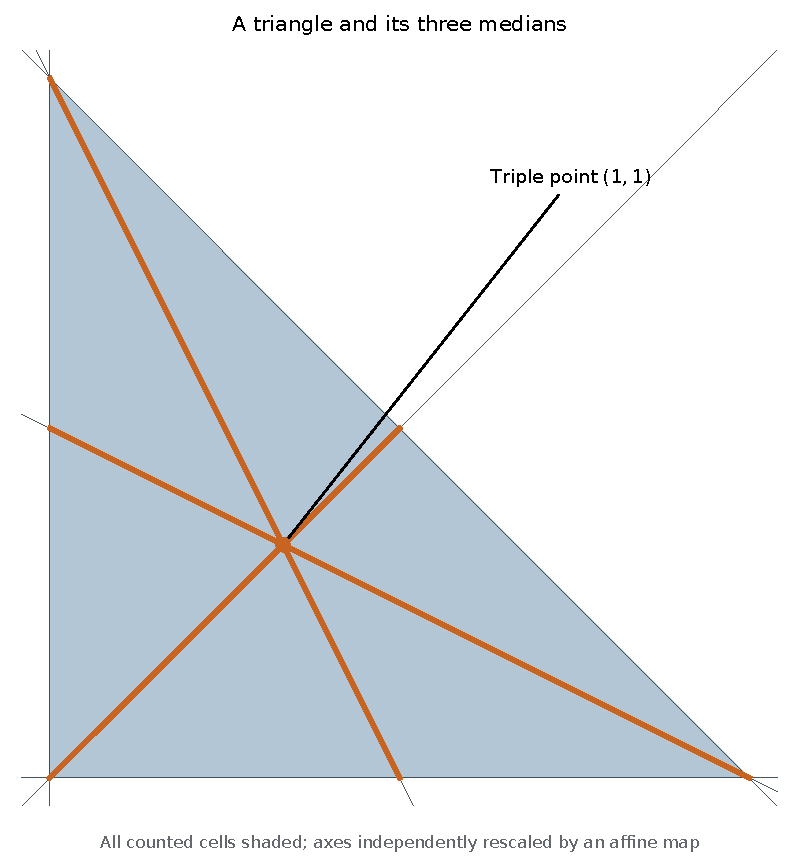
\includegraphics[width=0.75\textwidth]{figures/shared-fan.pdf}
\caption{The exact arrangement~\eqref{upper:median-lines}. Six triangular cells meet around the central triple point, and all six radial sides are shared. This refutes only a literal local incidence reading of the shared-pair statement in Cl\'ement--Bader's Lemma~1; it does not refute their final upper theorem. The figure is newly generated from the integer equations.}
\label{fig:shared-fan}
\end{figure}

The \texttt{SharedFan} module proves the real geometric facts: each designated triangle has nonempty uncut interior, the six interiors are pairwise disjoint, the radial segments are distinct and elementary, and each is a side of two distinct triangles. The proof uses ordinary kernel checking.

This matters when interpreting the Cl\'ement--Bader proof. Its local shared-pair sentence cannot literally bound all shared segments incident to a multiple point by two. An intended assignment of each shared side to one endpoint would be a different assertion requiring global justification. The example has only six triangles, below the reported seven-triangle upper bound at order six; it is therefore not a counterexample to that upper theorem. The present paper leaves that distinction explicit and uses the separate $D_1,D_2$ accounting instead.

Nor can one justify a simple upper bound merely by perturbing every multiple point. For a retained two-triple-point Maiorana $14{:}54$ witness, the four local generic resolution types have triangle counts $52,52,53,52$. These counts were checked with exact arithmetic; they are finite experimental evidence, not a new Lean theorem classifying all perturbations. They demonstrate why a universally nondecreasing smoothing argument needs more than the existence of a small generic perturbation. Our global upper argument never assumes such monotonicity.

\subsection{Actual arrangement extraction and simple upper theorems}
\label{upper:simple-actual}

The formal inventory is now built from an actual finite injective family
of certified triangles in $n\ge2$ pairwise nonparallel lines. It may
be a proper subset of all triangular cells. The quantities $U,D_1,D_2$
are defined relative to this selected family. The cell theorem proves
interior disjointness, and the side-emptiness theorem proves that each
side has consecutive endpoints on its supporting line.

An unordered endpoint pair represents one geometric side. At most two
pairwise interior-disjoint nondegenerate triangles can share that side:
three would put two on the same side of its support, forcing their
interiors to overlap near an interior base point. Counting triangle-side
incidences therefore gives $3T=E-U+D_1+D_2$. Pair counting proves
$\sum r(r-1)t_r=n(n-1)$ and the actual consecutive-edge inventory gives
$E=n(n-2)-S$. Thus
\begin{equation}
 \delta=S+U-D_1-D_2
 \label{upper:actual-identity}
\end{equation}
is proved from geometry by
\sourcefile{Kobon/UpperEdgeInventory.lean}{\lean{certificate_defect_identity}};
capacity, incidence and edge cardinality are conclusions of the proof,
not assumed numerical identities.

\begin{theorem}[Actual clean-line charging and simple bounds]
\label{upper:actual-simple}
Let $n\ge4$ be even. For any pairwise nonparallel real arrangement and
finite injective certified triangle family,
\begin{equation}
 n-h\le2U+D_1.
 \label{upper:actual-charging}
\end{equation}
For every simple arrangement with $T$ certified triangular cells,
\begin{equation}
 3T\le n(n-2)\quad(n\ge2),\qquad
 6T\le n(2n-5)\quad(n\ge4\text{ even}).
 \label{upper:actual-simple-bounds}
\end{equation}
\end{theorem}

\begin{proof}
The parity proof of Lemma~\ref{upper:clean-charge} can also be organized
as an odd-cardinality matching contradiction, which is the formal route.
A clean line has exactly $n-1$ distinct crossings. One common open
half-plane contains a further crossing on every transverse support.
Choose in that half-plane the consecutive bounded segment incident to
each clean-line crossing. Existence is obtained from the nearest actual
intersection, with the bounded-side and uniqueness lemmas handling
both signs.

If every chosen edge had degree one in the certified triangle family,
its unique triangle would have its base on the clean line: at an ordinary
crossing a triangle must use one of the two incident supports. Consecutive
edge uniqueness and interior disjointness then make these bases a
disjoint two-element cover of the clean-line crossings. Such a cover
has even cardinality, contradicting $n-1$ odd. Hence some incident
bounded edge has degree zero or two. A degree-two edge has a multiple
other endpoint by the shared-side lemma, so it is counted by $D_1$.

Choose one resulting charge for each clean line. A fixed ordinary
endpoint of an edge determines at most one clean transverse line.
An unused edge has at most two such endpoints and receives at most two
charges; a $D_1$ edge has exactly one ordinary endpoint and receives
at most one. This proves \eqref{upper:actual-charging}. The extraction,
choice and fiber bounds are all in
\proofref{Kobon/UpperCleanCharging.lean}{100}{\lean{certificate_clean_line_budget}},
using \lean{UpperCleanHalfplane}, \lean{UpperCleanEdges},
\lean{UpperCleanPairing} and \lean{UpperCleanCover}. No charge-existence
or pairing premise remains.

For a simple arrangement the core is empty, so $S=D_1=D_2=h=0$.
Equation~\eqref{upper:actual-identity} gives $3T=n(n-2)-U$, proving the
first bound. In the even case $n\le2U$, so
$6T=2n(n-2)-2U\le n(2n-5)$.
The \lean{SimpleLowerBound} versions extract the injective finite family
from its duplicate-free triangle list. These are
\sourcefile{Kobon/UpperSimpleOptimality.lean}{\lean{simple_lower_bound_upper}}
and
\sourcefile{Kobon/UpperEvenSimpleOptimality.lean}{\lean{simple_lower_bound_even_upper}}.
\end{proof}

The integer floor forms follow immediately. These classical inequalities
retain their earlier attribution, including Blanc's even parity bound.
Their contribution here is a complete real-geometric formalization with
standard logical axioms only. In particular, the retained simple
$44:608$ certificate attains $\lfloor44(88-5)/6\rfloor=608$; this
proves simple optimality at that order, not unrestricted optimality.
Theorem~\ref{upper:actual-simple} does not justify applying the even
polynomial to nonsimple witnesses such as $14:54$.

\subsection{Extremal fans and strengthened local restrictions}
\label{upper:extremal-fans}

\begin{theorem}[Equality structure of a supplied cyclic fan]
\label{upper:extremal-structure}
Consider actual local sector data at an $r$-fold point, $r\ge3$, satisfying
the cyclic order, antipodality, triangle and ordinary-endpoint conditions
of \lean{UpperFan.Sectors}. If $d_1=2r-3$, every sector is triangular
and $d_2=3$. Consequently,
\begin{equation}
 d_2\le2\Longrightarrow d_1\le2r-4,
 \qquad 3d_1+d_2\le6r-8+2e,
 \label{upper:extremal-weight}
\end{equation}
where $e=1$ when $d_1=2r-3$ and $e=0$ otherwise.
\end{theorem}

\begin{proof}
The no-long-run property from Lemma~\ref{upper:no-long-run} holds for
the selected ordinary-ended shared rays. If a sector were missing,
both bounding rays would be absent from that selected set. The cyclic
window count with these adjacent omissions strengthens its cardinality
bound to $2r-4$. Thus the extremal case has every sector present; all
$2r$ rays are then shared. Subtracting $d_1=2r-3$ gives $d_2=3$.
If $d_2\le2$, equality in the old bound is therefore impossible.
In the nonextremal case,
$3d_1+d_2=2d_1+(d_1+d_2)\le2(2r-4)+2r$; in the extremal case its
value is $6r-6$. These give \eqref{upper:extremal-weight}.
The exact proofs are
\proofref{Kobon/UpperFan.lean}{171}{\lean{all_sectors_of_extremal}},
\proofref{Kobon/UpperFan.lean}{187}{\lean{core_shared_card_eq_three_of_extremal}}
and \proofref{Kobon/UpperFan.lean}{227}{\lean{weighted_local_bound}}.
\end{proof}

This strengthens the previous manuscript's local hypothesis $d_2\le1$
to $d_2\le2$. The formerly supplied local interface is now extracted
from every actual core, as described below. A supported extreme core
cannot carry the full extremal fan
when its core-ended rays are identified with points in the supporting
closed half-plane (\lean{UpperFanSupport} and
\lean{UpperCoreBoundary}). Also, two full extremal triple fans cannot
be adjacent across the same matched elementary side with its two
neighboring certified triangles (\lean{UpperTripleFan}). The latter
uses the actual coincident endpoints and opposing adjacent sectors;
an arbitrary pair of abstract fan records need not supply that matching.
The completed arrangement wrapper derives it from the original selected
triangle occurrences, rather than assuming compatible abstract records.

\subsection{Actual fan extraction, matching and global assembly}
\label{upper:actual-global}

At each core the development orders the actual supporting directions by
an admissible affine chart, appends their opposite representatives, and
obtains a cyclic list of $2r$ nonzero rays. Consecutive selected triangle
sectors determine actual side endpoints. Simplicity of the elementary
segment inventory identifies a shared ray with its unique ordinary or
core endpoint, and injectivity of the selected triangle labels identifies
its two neighboring cell occurrences. Thus the local ordinary and core
ray counts equal $d_1(v)$ and $d_2(v)$, rather than supplied numerical
surrogates. The actual local bound is
\proofref{Kobon/UpperOpenMathActualFans.lean}{197}{\lean{certificate_local_fan_bound}};
matching along a shared elementary edge is
\proofref{Kobon/UpperOpenMathActualMatching.lean}{22}{\lean{certificate_neighbor_matching}}.
The geometric no-long-run and extremal conclusions above now apply to
these extracted records at every core.

Double counting their actual side incidences gives
$\sum_vd_1(v)=D_1$ and $\sum_vd_2(v)=2D_2$. In particular, the
weighted sum and exceptional-fan corrections no longer require a global
fan premise. The result is assembled in
\proofref{Kobon/UpperOpenMathGlobalFans.lean}{78}{\lean{certificate_weighted_fan_sum}}
and \proofref{Kobon/UpperOpenMathGlobalFans.lean}{204}{\lean{certificate_defect_even}}.
This completes the formal geometric scope of
Proposition~\ref{upper:weighted} and its higher-multiplicity corollary.
The previously conditional refined budget is now an actual theorem:
\begin{equation}
 2\delta\ge n+2S-7I+8q-2e+D_2,
 \label{upper:refined-conditional}
\end{equation}
where $e$ counts full extremal fans with ordinary degree $2r-3$.
The stronger boundary-sensitive assembly proves the two-core theorem
and the three-core estimate with their actual geometry, in
\proofref{Kobon/UpperOpenMathBoundaryBudgets.lean}{128}{\lean{certificate_three_core_upper}}
and \proofref{Kobon/UpperOpenMathBoundaryBudgets.lean}{137}{\lean{certificate_two_core_upper}}.
The former gives, when $q\le3$ and $n=2m$,
\begin{equation}
 \delta\ge m-6,\qquad T\le\floor{m(4m-5)/3}+2,
 \label{upper:three-core-conditional}
\end{equation}
equivalently $6T\le n(2n-5)+12$. The retained labels record the historical
conditional statements; their arrangement extraction is now complete.
For $q\le1$, or $q\le2$ with at most one triple core, the sharper
rounding is $6T\le n(2n-5)+2$, proved by
\sourcefile{Kobon/UpperOpenMathSparseUpper.lean}{\lean{UpperOpenMathSparseUpper}}.
These are restricted numerical consequences at every even order.

Several independent exact resources retain geometry that earlier budgets
discarded. Let $C$ count core endpoints of bounded nonshared elementary
sides, and $R_c$ count unbounded rays at cores. Actual first/last vertex
flags give
\begin{align}
 D_1+2D_2+C+R_c&=2I,\\
 2\delta&=2\sum_{r\ge3}r(r-3)t_r+2U+C+R_c-D_1.
 \label{upper:ray-identities}
\end{align}
The source \lean{UpperOpenMathRayResources} proves both identities.
The actual shared-core graph has core vertices and $D_2$ edges, including
isolated vertices in its component partition. Its component hull points
consume at least two nonshared or ray resources each. If $b_h$ is the
sum of the numbers of supporting hull points of the individual components,
then the completed hull estimate is
\begin{equation}
 2\delta\ge2U+2\sum_{r\ge3}r(r-4)t_r+3q+3b_h.
 \label{upper:component-hull}
\end{equation}
It follows from separately bounding ordinary sharing and total sharing
at each supported core; see
\proofref{Kobon/UpperOpenMathComponentHullDeficit.lean}{86}{\lean{certificate_component_hull_deficit}}.
If all core multiplicities are at least $R\ge4$, this gives
$6T+(2R(R-4)+3)q+3b_h+2U\le2n(n-2)$.
The cases $R=4,5$ retain penalties $3q,13q$, respectively.
These are structural estimates, not a formula for the unrestricted maximum.

\subsection{Degree-free structural bounds and their local counts}
\label{upper:degree-free}

All statements in this subsection concern $n\ge2$ pairwise nonparallel
real lines and an arbitrary finite injective family of certified triangular
cells. All core, side and component counts are extracted from that family.
At a core put $a=d_1$, $d=d_2$. A \emph{marked port} is a shared core ray
whose two neighboring shared rays end at ordinary vertices. Let $m$ be
the number of such ports. In the all-triple class each marked edge reaches a poor fan,
with $a\le1$ and $a+d\le2$, and a shared edge receives at most one source
marker. Define
\begin{align*}
 \Delta&=\sum_{r\ge4}r(r-4)t_r,\\
 A_{\rm all}&=\#\{\text{triple cores with }(a,d)=(2,4)\},\\
 A_0&=\#\{\text{triple cores with }(a,d,m)=(2,4,0)\},\\
 B_{15}&=\#\{\text{triple cores with }(a,d)=(1,5)\}.
\end{align*}
Use $A_s,B_s$ for the corresponding unmarked two-cap and one-cap
counts in component $s$. The following component bound has no degree,
size or multiplicity restriction.

\begin{theorem}[Mixed and marked component defects]\label{upper:mixed-degree-free}
For arbitrary core multiplicities,
\begin{equation}
 \delta+A_{\rm all}+\sum_s\ceil{B_s/2}\ge U+c+\Delta.
 \label{upper:mixed-component}
\end{equation}
Its complementary doubled form is
$2\delta+2A_{\rm all}+B_{15}\ge2U+c+2\Delta$.
If every core is triple, the first formula strengthens to
\begin{equation}
 \delta+A_0+\sum_s\ceil{B_s/2}\ge U+c.
 \label{upper:marked-component}
\end{equation}
\end{theorem}
\begin{proof}
The actual cap budgets, and in the all-triple case the marked-edge budgets,
pay extremal and partial sources
against poor endpoint capacities. Higher multiplicity pays through its
quadratic surplus, without assuming that higher extremal fans are
independent. On each nonempty closed component the adjusted paid cost
is strictly positive. Equality in the finite budget restricts the local
fan types: balanced two-cap fans, marked full two-cap fans and full
zero-cap fans remain, with the residual full types added in the later
paid equality case. A closed balanced subset forces a three-cycle by
matching its actual triangle identities. The third normalized cap axis
would have to contain a point beyond both endpoints of one elementary
core side, which is impossible.

The remaining full-fan cluster cannot be finite. A full zero-cap center
is surrounded by cluster neighbors; a marked two-cap center has an
actual opposite continuation through a poor fan to another cluster point.
A point maximizing squared norm in this finite cluster cannot satisfy
either property. In the mixed case a finite supporting line excludes the
closed higher/extremal cluster, and the normalized remaining triple
mixture is handled by the same occurrence matching. Integer rounding
of the strictly positive paid cost gives one unit per component.
The final roots are
\proofref{Kobon/UpperOpenMathMixedCurvatureBound.lean}{41}{\lean{certificate_mixed_curvature_component_bound}}
and \proofref{Kobon/UpperOpenMathPaidCurvatureBound.lean}{116}{\lean{certificate_component_half_penalty_bound}}.
No planar graph, supplied fan, convex-hull oracle or unproved aggregate
identity is a hypothesis of these arrangement wrappers.
\end{proof}

The residual corrections cannot simply be dropped. Actual unmarked
full $(2,4)$ fans exist; full $(1,5)$ fans may be adjacent. In particular,
exact rational witnesses have an unmarked $(2,4)$ core adjacent to a
marked $(2,4)$ core at eight lines and twelve triangles, and to a full
$(1,5)$ core at nine lines and sixteen triangles. Therefore an independence
argument for all negative local types would be false.

\subsection{Recipient geometry and the final all-triple gain}
\label{upper:source-free}

Let an \emph{antipodal source} mean a core counted by $A_0$. Its two
ordinary shared rays are opposite. Actual triangle matching proves that
two such sources cannot share a side, nor can a source meet an unmarked
balanced $(2,2)$ fan. Each source has at least two nonfull neighbors;
its two cap flanks cannot both meet full triple fans. Two distinct sources
have at most two common actual core neighbors. The latter theorem allows
arbitrary multiplicities at the other cores: opposite-pair extraction
would otherwise force an intervening vertex on an elementary side or
crossing strict cevians inside such sides. This is
\proofref{Kobon/UpperOpenMathAntipodalThreeNeighbors.lean}{94}{\lean{certificate_common_neighbor_card_le_two}}.

In the all-triple class, a recipient of total shared degree at most four
has at most two source neighbors. For a one-cap $(1,3)$ recipient,
complete extraction of its five-sector chart strengthens this to at most
\emph{one}. Adjacent source tips contradict source independence; the
remaining six tip placements are excluded by support exhaustion,
ordinary-tip identification and opposite-ray continuation, with affine
area signs handling the separated positions. The actual endpoint is
\proofref{Kobon/UpperOpenMathN13ActualNoDouble.lean}{13}{\lean{certificate_n13_no_two_anti_neighbors}}.
A $(1,2)$ recipient similarly has a three-shared-ray run: two sources
would be adjacent or separated by the ordinary middle ray, whose
continuation is impossible. See
\proofref{Kobon/UpperOpenMathN12Recipient.lean}{152}{\lean{certificate_n12_anti_degree_le_one}}.
A partial $(2,1)$ recipient has no source neighbor, because its only core
edge reaches a poor fan while a source has ordinary shared degree two.
An actual $(1,3)$ recipient with a source neighbor also cannot maximize
an affine functional injective on a finite closed shared-core set containing
it. The extracted support contradiction is
\proofref{Kobon/UpperOpenMathN13ActualSupportExtreme.lean}{14}{\lean{certificate_n13_with_anti_not_max}}.
This restricts exposed equality profiles but does not by itself prove
strict positivity of every component.

Define the positive local counts
\[
 \begin{aligned}
 E_3&=\#\{a=3\},&\qquad P_{21}&=\#\{(a,d)=(2,1)\},\\
 N_{12}&=\#\{(a,d)=(1,2)\},& M_{22}&=\#\{(a,d)=(2,2),\ m\ge1\}.
 \end{aligned}
\]
These definitions in this subsection range over actual triple cores.
\begin{theorem}[Source-free triple defect with marked balanced gain]
\label{upper:final-m22}
If every actual core has multiplicity three, then
\begin{equation}
 2\delta+B_{15}\ge2U+3(E_3+P_{21})+N_{12}+M_{22}.
 \label{upper:m22-global}
\end{equation}
Equivalently,
$6T\le2n(n-2)+B_{15}-2U-3(E_3+P_{21})-N_{12}-M_{22}$.
There is no degree, component-size or source-count restriction.
\end{theorem}
\begin{proof}
The finite unit discharging rule charges antipodal-source edges against
the actual marked-port and recipient capacities. The $(1,3)$ restriction
removes its former double-recipient correction completely; the $(1,2)$
restriction leaves one positive unit, and the $(2,1)$ exclusion increases
its coefficient to three. These yield the completed N12 theorem
\proofref{Kobon/UpperOpenMathN12Curvature.lean}{99}{\lean{certificate_n12_source_free_defect_bound}}.

For the late additional term, marked outgoing edges and incoming
antipodal-source edges have disjoint opposite endpoint types. Both sets
lie in the actual incident core-edge inventory. Thus at every core
\begin{equation}
 m(v)+\deg(A_0,v)\le d(v).
 \label{upper:local-port}
\end{equation}
At a marked balanced core the local discharging weight is zero but
$m\ge1$; \eqref{upper:local-port} gives $m+x\le2$, hence $2m-x\ge1$.
This retains the extra unit counted by $M_{22}$. The local extraction is
\proofref{Kobon/UpperOpenMathLocalPortBudget.lean}{10}{\lean{certificate_marked_plus_anti_degree_le}},
and the global actual wrapper is
\proofref{Kobon/UpperOpenMathM22Curvature.lean}{117}{\lean{certificate_m22_source_free_defect_bound}}.
The finite weights, recipient geometry and actual wrappers all use only
standard logical axioms.
\end{proof}

The estimates developed on the way are retained as independently checked
intermediate resources. The half-curvature rule is
$2\delta+A_0+B_{15}\ge2U$; its first positive refinement is
$4\delta+2A_0+2B_{15}\ge4U+6E_3+5P_{21}$, improved to coefficient six
for $P_{21}$ after partial-recipient exclusion. The double-recipient rule
$2\delta+B_{15}+J_{13}\ge2U+3E_3+2P_{21}$ used the exact count of
$(1,3)$ double receivers; actual geometry now proves $J_{13}=0$.
The final global estimate dominates these global unit/half gains but
retains $B_{15}$. No unrestricted upper polynomial follows by omitting it.

\begin{figure}[tb]
\centering
\includegraphics[width=0.95\linewidth]{new-upper-profile-coefficients.pdf}
\caption{Coefficients in the earlier half-curvature inequality and the
final all-triple global estimate developed during 5--6 October. Both
are structural bounds for actual nonparallel arrangements. The bars
compare algebraic charges of local types; they do not assert that an
arbitrary collection of those types is geometrically realizable, and
are not a comparison with an unrestricted numerical upper bound.}
\label{fig:upper-coefficients}
\end{figure}

\begin{theorem}[Componentwise N12 portfolio]\label{upper:n12-hybrid}
Under the all-triple hypothesis, let $A_s,B_s,E_s,P_s,N_s$ be the
corresponding counts in the actual component $s$. Then
\begin{equation}
 \delta\ge U+\sum_s\max\left\{
 1-A_s-\ceil{B_s/2},\;
 \ceil{\frac{3E_s+3P_s+N_s-B_s}{2}}\right\}.
 \label{upper:n12-component}
\end{equation}
This score dominates the preceding half-gain and source-free component
scores. If each component satisfies $B_s+1\le3E_s+3P_s+N_s$, then
$\delta\ge U+c$.
\end{theorem}
\begin{proof}
Localize the actual discharging and strict paid-cost arguments to each
shared-core-closed component. The component contribution $H_s$ to
$\delta-U$ is integral. The paid theorem gives
$H_s\ge1-A_s-\ceil{B_s/2}$; the source-free N12 theorem gives the other
rounded score. Take their maximum \emph{before} summing over components.
Actual component partition and side double counting prove
$\delta-U=\sum_sH_s$. The final component endpoint is
\proofref{Kobon/UpperOpenMathClosedN12Curvature.lean}{282}{\lean{certificate_n12_source_free_hybrid_component_defect}};
its dominance is proved in the same module. The sufficient positive
profile is
\proofref{Kobon/UpperOpenMathPositiveProfileComponents.lean}{43}{\lean{certificate_positive_profile_component_defect}}.
\end{proof}
The $M_{22}$ strengthening in \eqref{upper:m22-global} is currently a
\emph{global} theorem. Equation~\eqref{upper:n12-component} is the separately
completed component portfolio; no componentwise M22 extension is claimed.

\subsection{Restricted graph classes and multiplicity consequences}
\label{upper:classes}

The cap budgets themselves require no graph restriction. In the
all-triple class they give
\[
 D_1+2E_3+P_{21}\le2q,\qquad
 \delta\ge U+q-D_2+2E_3+P_{21},
\]
in \proofref{Kobon/UpperOpenMathTripleCapBudget.lean}{57}{\lean{certificate_triple_cap_budget}}.
For arbitrary multiplicities, define
$\mathcal A=\sum_{r\ge4}(r(r-4)+1)t_r$ and
$P_{\rm poor}=\sum_{v\text{ poor triple}}d(v)$, where poor means
$a\le1$ and $a+d\le2$. The mixed weighted budget is
\[
 3D_1+3q+3\mathcal A+2P_{\rm poor}\le3S,\qquad
 3\delta\ge3(U+q-D_2+\mathcal A)+2P_{\rm poor}.
\]
It is \proofref{Kobon/UpperOpenMathMixedCapBudget.lean}{53}{\lean{certificate_mixed_weighted_budget}}.
An order-four, -five or -six core contributes respectively one, six
or thirteen to $\mathcal A$. These contributions pay triple sources
without assuming that higher extremal fans are independent.

\begin{theorem}[Component and forest classes]\label{upper:class-corollaries}
For the same actual arrangement and triangle-family semantics:
\begin{enumerate}[label=(\roman*)]
\item If every core has shared-core degree at most three, then
$\delta\ge U+c+\Delta$, with arbitrary multiplicities.
\item At degree at most four, the bound is
$\delta+A_{\rm all}\ge U+c+\Delta$.
\item If each actual component has at most five vertices, then
$\delta\ge U+c+\Delta$, with arbitrary total core count and multiplicities.
\item For an actual forest, put
$\mathcal A=\sum_{r\ge4}(r(r-4)+1)t_r$ and let
$P_{\rm poor}=\sum_{v\text{ poor triple}}d(v)$. Then
$3\delta\ge3(U+c+\mathcal A)+2P_{\rm poor}$.
For an all-triple forest the separate cap budget gives
$\delta\ge U+c+2E_3+P_{21}$.
\end{enumerate}
\end{theorem}
\begin{proof}
At degree at most three, adjusted component cost is nonnegative. Its
zero case leaves a closed extremal cluster or a balanced two-cap cluster;
finite supporting geometry excludes the former and actual cycle geometry
the latter, giving strict integer cost. The degree-four version retains
full two-cap corrections. In a component of at most five vertices, a
full two-cap center and its four neighbors exhaust the component.
Opposite radial segments and ordinary cap tips block outer diagonals.
The remaining endpoint weights pay more than the center's negative
weight; mixed outer multiplicities supply their adjusted surplus.
Both antipodal and non-antipodal full two-cap shapes are handled.
These are
\proofref{Kobon/UpperOpenMathMixedDegreeThree.lean}{158}{\lean{certificate_mixed_degree_three_component_bound}},
\proofref{Kobon/UpperOpenMathMixedDegreeFour.lean}{169}{\lean{certificate_mixed_degree_four_component_bound}},
and \proofref{Kobon/UpperOpenMathMixedFiveCoreComponents.lean}{96}{\lean{certificate_mixed_five_component_bound}}.

For a forest, the actual component trees prove $D_2+c=q$.
The mixed weighted cap budget
$3\delta\ge3(U+q-D_2+\mathcal A)+2P_{\rm poor}$ gives the result.
The all-triple budget retains $D_1+2E_3+P_{21}\le2q$ before substitution
in the exact defect identity. The forest endpoints are
\proofref{Kobon/UpperOpenMathForestBudget.lean}{73}{\lean{certificate_mixed_forest_weighted_bound}}
and \proofref{Kobon/UpperOpenMathForestBudget.lean}{49}{\lean{certificate_triple_forest_bound}}.
No degree bound is required for the forest statements.
\end{proof}

A closed all-triple component of at most seven vertices contains at most
one antipodal source: two nonadjacent sources need two four-element
neighbor sets among at most five other vertices, contradicting the
at-most-two-common-neighbor theorem. The single-source charging rule gives
$\delta\ge U+\sum_s\ceil{(3E_s+2P_s-B_s)/2}$ in that class; an adaptive
maximum retains the stronger rule separately in each applicable component.
This does not remove $B_s$ or prove $\delta\ge U+c$ for all seven-core
components. The final unrestricted N12 portfolio is retained alongside
these earlier source-sensitive results.

The mixed high-multiplicity consequences also have actual formal proofs.
All multiplicities at least four imply $3T\le n(n-2)$.
At even order, multiplicities at least six give
$6T+6q\le n(2n-5)$; the sharper five-or-higher boundary theorem gives
$12T+5q+\min(q,3)\le2n(2n-5)$.
The proofs are in \lean{UpperOpenMathMultiplicity},
\lean{UpperOpenMathHighMultiplicityHull} and \lean{UpperOpenMathBoundaryBudgets}.
These restricted numerical formulas are not replacements for control of
triple and quadruple cores in the unrestricted problem.

\subsection{Parity tokens, equality attribution and remaining limits}
\label{upper:tokens}

The new parity extraction can charge every cut line in an even all-triple
arrangement, rather than only clean lines. Ordinary crossings there have
odd cardinality. The base cover either fails degree one on a transverse
segment or ends a positive triangle base at a core. Separately accounting
for these two modes gives the safe actual bound
\begin{equation}
 n\le2U+2D_1+C\qquad(n\ge4\text{ even, all cores triple}).
 \label{upper:all-line-parity}
\end{equation}
Its proof is in \lean{UpperOpenMathOrdinaryGlobalCharge}. The second $D_1$
is necessary: a four-line pencil-plus-cap witness has $U=0,D_1=1,C=2$,
so replacing $2D_1$ by $D_1$ would give the false $4\le3$.
The conjectural trade-off $n\le2U+D_1+R_c+2$, together with
$C\ge2D_1$, would yield the corrected even bound
$6T\le n(2n-5)+2$ in the all-triple class. Neither conjectural resource
rule is assumed here. Without the correction two, the known $38:450$
witness has token total 36; with correction two the rule still fails for
mixed multiplicities, where a $14:52$ witness has shortfall three.

Cl\'ement--Bader already stated that exact Tamura equality forces a
simple configuration~\cite{clementbader2007}. The quantitative penalties
and restricted equality corollaries above are independently checked
mechanisms in explicit scopes, not a claim of first discovery of that
broad conclusion. The wrong-ray/shared-apex mechanism also has prior local
arguments in Srirangam's notes~\cite{srirangam2026}; their actual fan
extraction, extended partial-fan scopes and global weighted assembly are
separate developments here. Source priority for the quantified component
penalties requires further comparison.

An exact phase-zero F\"uredi--Pal\'asti witness with eight lines has seven
triple cores, fourteen triangles and fifteen shared sides, refuting the
auxiliary general shortcut $D\le2q$. At eighteen lines its exact profile
is $q=46,D_1=15,D_2=105$. An eleven-line witness has adjacent order-five
extremal full fans, so higher extremal independence is also false.
These retained exact external counterexamples invalidate specified
charging shortcuts, not the final numerical conjectures in which those
shortcuts were used. A seven-vertex kernel-checked abstract half-charging
example is sharp for its finite relaxation but unrealizable: its two
sources would have the same four neighbors. It therefore identifies
missing geometry rather than sharpness for real Kobon arrangements.

A finite projective chart theorem now removes parallel pairs while
preserving a chosen finite set of actual bounded triangles. It requires
distinct projective lines and nonparallel supporting pairs for each
triangle; the old polynomial predicate alone is not used on a parallel
support pair. The endpoint
\proofref{Kobon/OpenMathParallelElimination.lean}{199}{\lean{arbitrary_iff_lowerBound}}
links the arbitrary and nonparallel lower-witness models. Class properties
and local profile counts must still be checked in the transformed chart;
this does not silently extend an all-triple theorem to every parallel
arrangement. The remaining general upper task is mathematical control
of residual profiles and the ordinary-end token trade-off, rather than
unfinished extraction of the fans already used above.
